\documentclass[11pt]{article}
\usepackage[margin=1in]{geometry}
\usepackage{fancyhdr}
\usepackage{graphicx}
\usepackage[utf8]{inputenc}
\usepackage[T1]{fontenc}
\usepackage{cite}
\usepackage{xcolor}
\usepackage{listings}
\usepackage{pdfpages}
\usepackage{import}
\usepackage{listings}

\pagestyle{fancy}
\fancyhead{}
%\fancyfoot{}
	\fancyhead[L]{Commande de robot par BCI}
\fancyhead[R]{Rafael, Mathieu, Heloise}
%\fancyhead[C]{\thepage}

\renewcommand{\contentsname}{\huge{\textbf{Table des matières}}}

\lstdefinestyle{DOS}
{
    backgroundcolor=\color{black},
    basicstyle=\scriptsize\color{white}\ttfamily
}


\begin{document}

%Title

\begin{titlepage}
\begin{center}

\includegraphics[scale=0.5]{CentraleSupelec.jpeg}\\
\vfill
\line(1,0){400}\\[1mm]
\huge{\textsc{\textbf{Rapport TL SIR Commande de robot par interface cérébrale}}}\\[3mm]
\Large{\textbf{- Rafael ELLER CRUZ, Mathieu DAVIET, Heloise HUYGHUES DESPOINTES-}}\\[1mm]
\Large{promo 2018}\\[1mm]
\line(1,0){400}\\[1mm]

\vfill

\end{center}
\end{titlepage}

%%%Table of contents%%%

\tableofcontents
\thispagestyle{empty}
\cleardoublepage

\pagenumbering{arabic}

%%%Introduction%%%
\setcounter{page}{1}
\section{Introduction}

Lors de ses 11 séances de TL d'approfondissement, nous avons eu l'occasion de réaliser la commande d'un robot Khepera à partir de signaux provenant d'une interface cerveau machine (BCI). Ce projet nous a permis de mettre en pratique les connaissances que nous avons acquises lors des cours de la majeure Systèmes Interactifs et Robotiques et plus particulièrement celles des cours de Modélisation et Analyse Spectrale, Robotique autonome et Programmation C++.\\

Deux robots Khepera, un système d'acquisition cérébrale et 3 signaux pré-enregistrés ont été mis à notre disposition pour ce projet. Le robot ne sera commandé que par 4 ordres: rester immobile, tourner à droite, tourner à gauche et avancer.\\

Notre travail à travers les séances et dans ce rapport est décomposé en 2 grandes étapes: l'extraction des commandes sur les signaux BCI que nous avons effectué principalement sous Matlab et le contrôle du robot grâce au framework ROS et à Python.


\cleardoublepage

%%%Extraction de la commande%%%

\section{Étapes amenant à l'extraction de la commande du robot à partir des signaux cérébraux}

\subsection{Le signal d'entrée}

Le signal de commande que l'on va être amené à analyser en entrée du système correspond au signal en sortie de la BCI. Dans le cadre de ce TL, 3 signaux pré-enregistrés à une fréquence de 256Hz nous ont été fournis et peuvent être rejoués à volonté. Pour chaque période de temps, les signaux enregistrés possèdent deux valeurs correspondant chacune à un canal du capteur. Nous aurions pu effectuer nos propres enregistrements à l'aide d'un capteur BIOSEMI à 2048Hz mais par manque de temps, nous nous sommes concentrés sur les signaux déjà enregistrés. \\

Le signal en sortie de la BCI est influencé par trois plaques clignotant respectivement autour de 7.5Hz, 11Hz et 13.5Hz. Lorsque l'expérimentateur regarde l'une des plaques à une fréquence donnée, cette fréquence se répercute dans l'émission de ses signaux cérébraux et se retrouve dans le signal récupéré par la BCI. Chacune de ces plaques clignotantes correspond à un ordre particulier. L'expérimentateur doit regarder la plaque clignotant à 7.5Hz si il veut que le robot tourne à gauche, celle clignotant à 11Hz si il veut que le robot avance, celle clignotant à 13.5Hz si il veut que le robot tourne à droite et ne regarder aucune plaque si il veut que le robot s'arrête.

\begin{figure}[!h]
	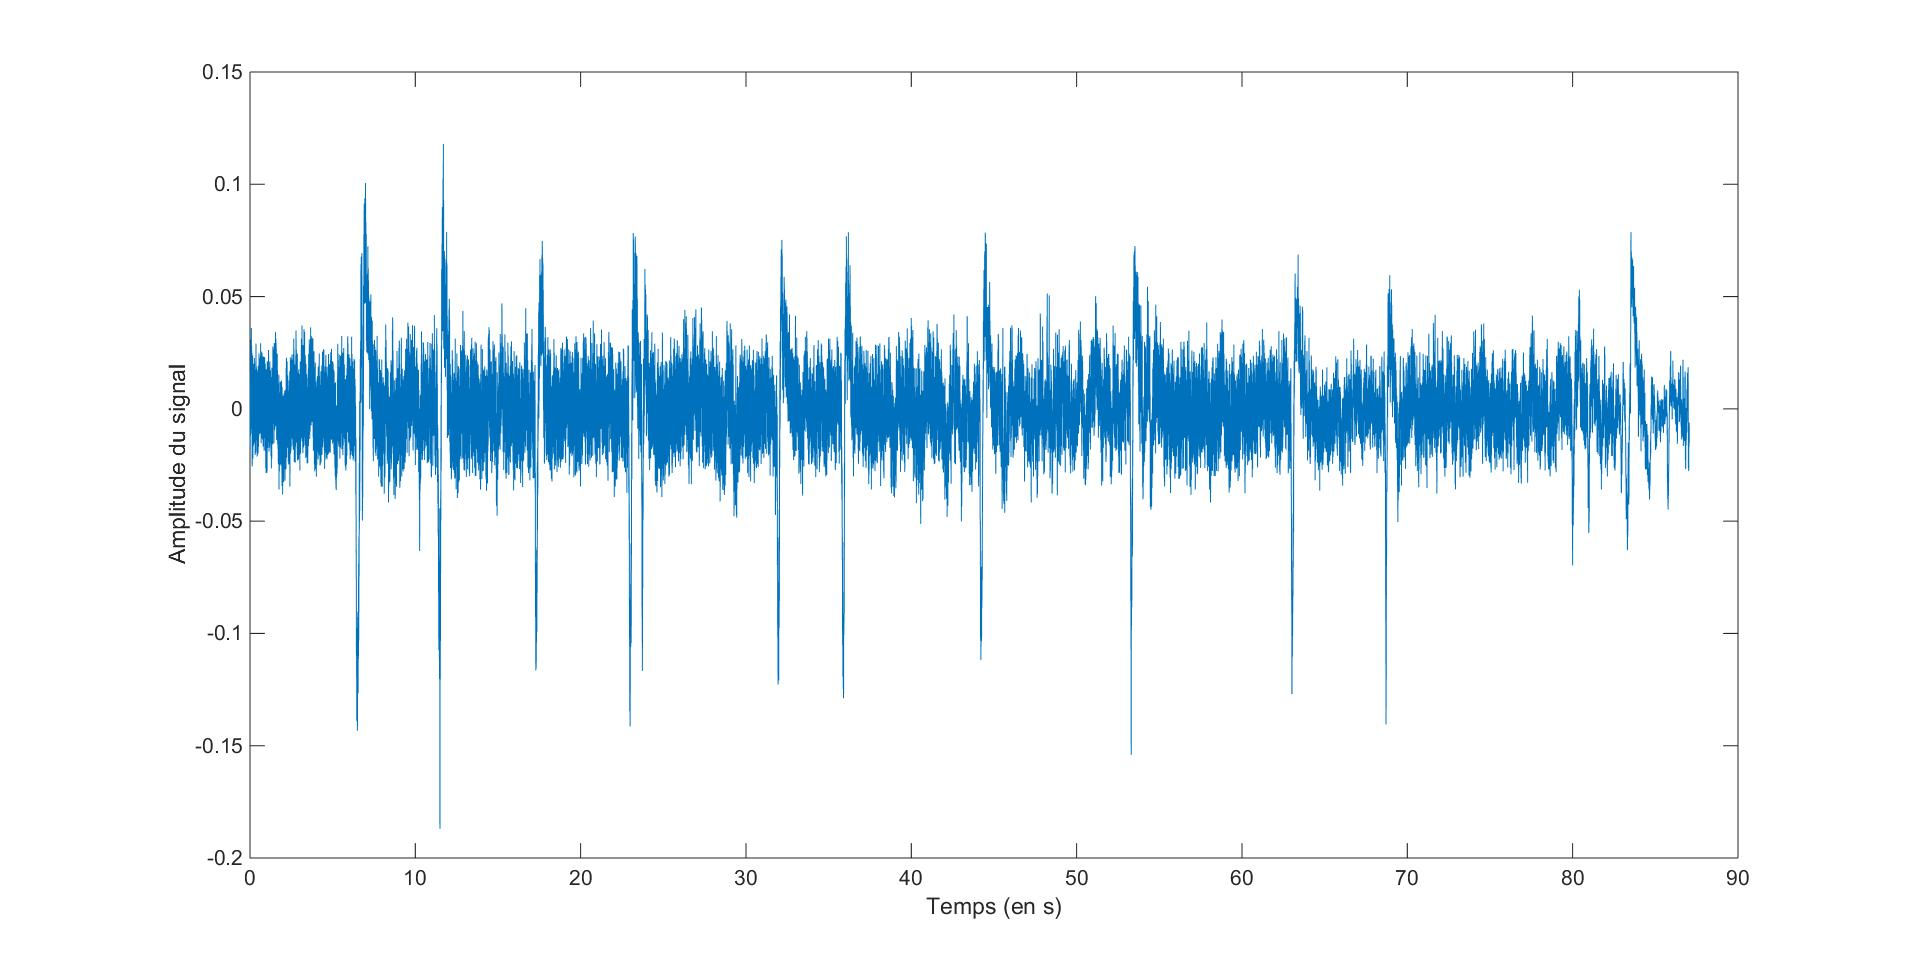
\includegraphics[scale=0.25]{images/signalBCIinit.jpg}
	\caption{Signal brut en sortie de la BCI enregistré}
	\label{fig:duck}
\end{figure}

Pour faciliter l'exploitation des résultats nous avons appliqué un pré-processing aux signaux enregistrés. \\

Tout d'abord, les signaux enregistrés sont bi-canaux. Ainsi, pour qu'ils soient plus faciles à manipuler par la suite, nous les avons transformés en signaux monocanal correspondant à la moyenne des deux canaux. \\


Ensuite, le problème est que les signaux enregistrés ne possèdent pour l'instant que les valeurs du capteur en fonction du temps. Les labels indiquant quels ordres ont été donné dans le temps ne sont disponibles que de manière écrite dans le sujet. Pour faciliter la modélisation et l'optimisation de la commande de robot par la suite, nous avons ajouté une deuxième colonne à chaque signal monocanal enregistré correspondant à l'ordre attendu en fonction du temps. Pour ce faire, nous avons associé un nombre à chaque ordre: 0 pour l'ordre ne rien faire, 1 pour l'ordre d'avancer, 2 pour l'ordre de tourner à droite et 3 pour l'ordre de tourner à gauche. L'ajout du label automatiquement nous permettra par la suite d'évaluer le taux d'erreur que nous commettons par rapport aux ordres attendus dans le but d'évaluer l'efficacité du traitement du signal que nous effectuerons.

\begin{figure}[!h]
	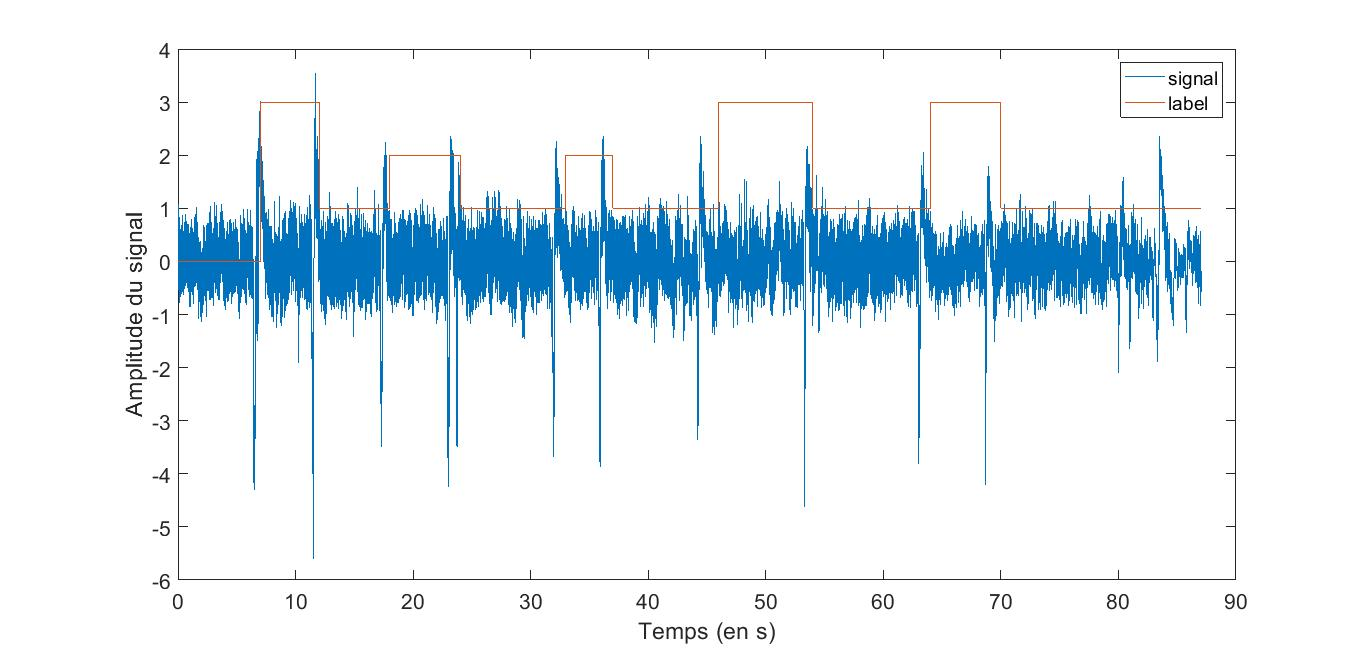
\includegraphics[scale=0.35]{images/signalBCIlabele.jpg}
	\caption{Signal brut monocanal labellisé}
	\label{fig:duck}
\end{figure}

\cleardoublepage


\subsection{Etapes pour l'extraction de la commande à partir du signal}

Comme on peut le constater sur la figure 1, le signal a besoin d'être traité pour pouvoir être exploité par la suite. La première étape va consister à extraire du signal de départ 3 signaux autour des fréquences qui nous intéresse à savoir 7.5 Hz, 11Hz et 13.5Hz. Pour effectuer cela nous utilisons 3 filtres passe-bande dont les paramètres sont la bande passante: $\Delta$ f, le gain: G et la fréquence centrale: fc. Les fréquences centrales correspond respectivement à 7.5Hz, 11Hz et 13.5Hz pour chacun des 3 filtres. Nous verrons par la suite le moyen par lequel nous avons optimisé les autres paramètres. Comme le montre la figure 3 ci-dessous, nous constatons que ce premier filtre nous permet déjà de distinguer les ordres donnés par l'expérimentateur via la BCI.

\begin{figure}[!h]
	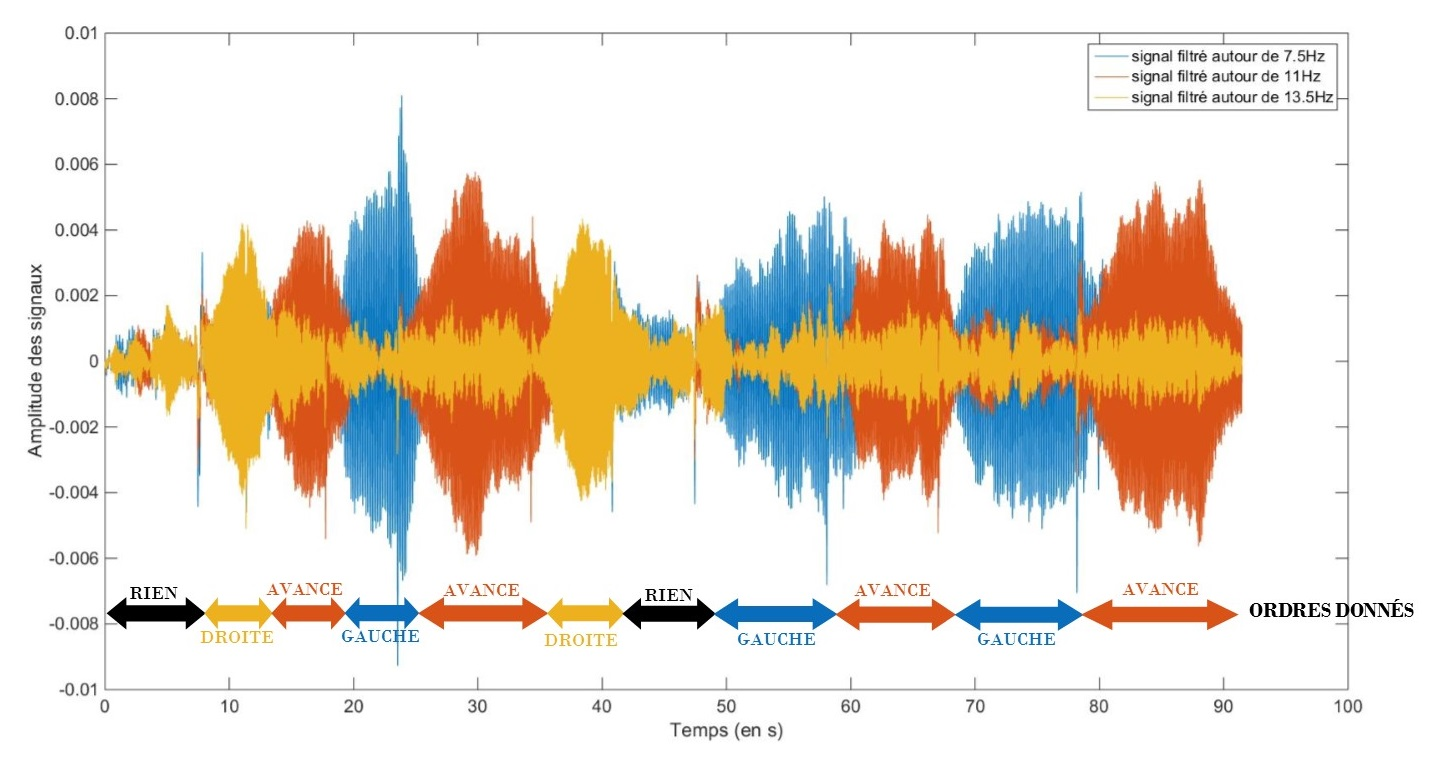
\includegraphics[scale=0.75]{images/Sigauxfiltreslables.jpg}
	\caption{Trois signaux en sortie du filtre passe bande centrés repectivement en 7.5Hz, 11Hz et 13.5Hz}
	\label{fig:duck}
\end{figure}

Malgré que le fait que l'on arrive à distinguer à l'œil nu les ordres à partir des 3 signaux en sortie des filtres passe-bande, il est nécessaire d'obtenir des signaux plus propres pour par la suite formaliser un processus de décision concernant la commande du robot. En effet, le signal est toujours sous forme sinusoïdale, ce qui n'est pas pratique pour calculer son amplitude à un moment précis. De plus, le signal est encore très sensible au bruit. Pour résoudre ces problèmes nous allons calculer la puissance lissée de chacun des 3 signaux.\\


\begin{figure}[!h]
	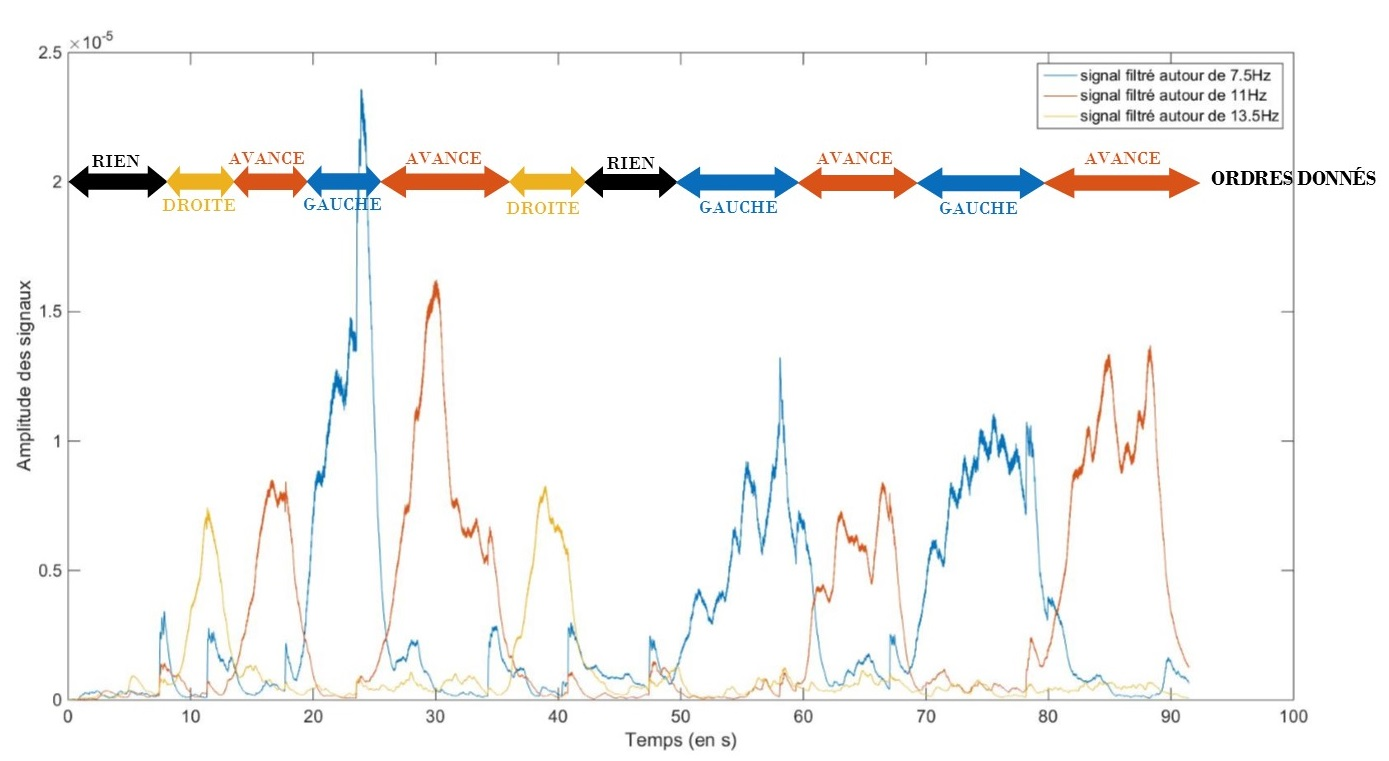
\includegraphics[scale=0.75]{images/puissancelissee.jpg}
	\caption{Trois signaux en sortie du filtre passe bande centrés respectivement en 7.5Hz, 11Hz et 13.5Hz}
	\label{fig:duck}
\end{figure}

Nous obtenons la puissance en mettant au carré notre signal, cela nous permet d'avoir un signal ne contenant que des valeurs positives. L'effet de lissage permet de réduire le bruit mais cela augmente l'inertie et diminue la résolution. Cet effet de lissage dispose d'un paramètre $ \alpha $ dont nous justifierons le choix par la suite. 
La puissance lissée nous permet ainsi d'obtenir des signaux exploitables par la suite pour commander le robot grâce à un processus de décision qui va être détaillé dans la suite du rapport. \\

Ensuite, dans la partie dédiée à la mise en pratique avec ROS, nous allons voir qu'il est nécessaire de mettre en place un buffer pour réduire la fréquence du système. Pour coller le plus possible à la réalité nous allons donc simuler ce buffer grâce à un filtre passe-bas appliqué à la puissance lissée. Cela nous permettra d'effectuer des simulations plus pertinentes. Les filtres passe-bas à les mêmes effets que le lissage de la puissance: diminution du bruit et augmentation de l'inertie.\\

Pour récapituler cette partie, un diagramme se trouve ci-dessous retraçant les différentes étapes par lesquelles passent le signal pour que l'on puisse en extraire un ordre. \\


\begin{figure}[!h]
	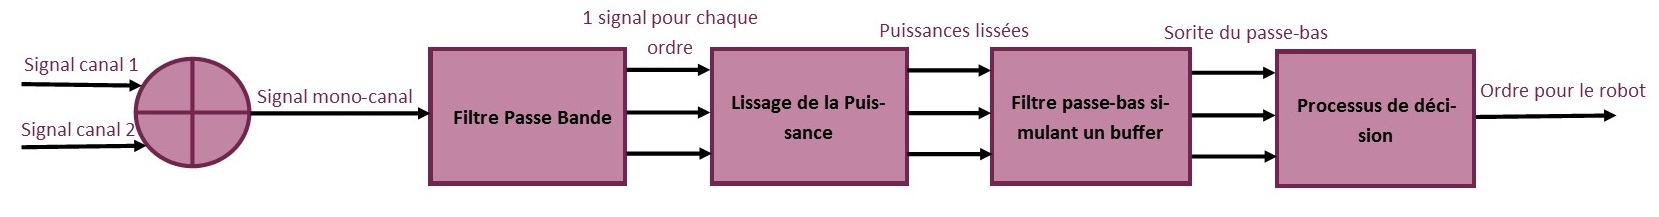
\includegraphics[scale=0.65]{images/diagramme.jpg}
	\caption{Récapitulatif de l'architecture nous permettant de prendre une décision quant à l'ordre à donner au robot}
	\label{fig:duck}
\end{figure}



\cleardoublepage


Nous avons donc tenté de comprendre pourquoi nous obtenons de si mauvais résultats pour le premier enregistrement. Nous avons fait plusieurs hypothèses et nous avons trouvés deux explications. \\

\begin{figure}[!h]
	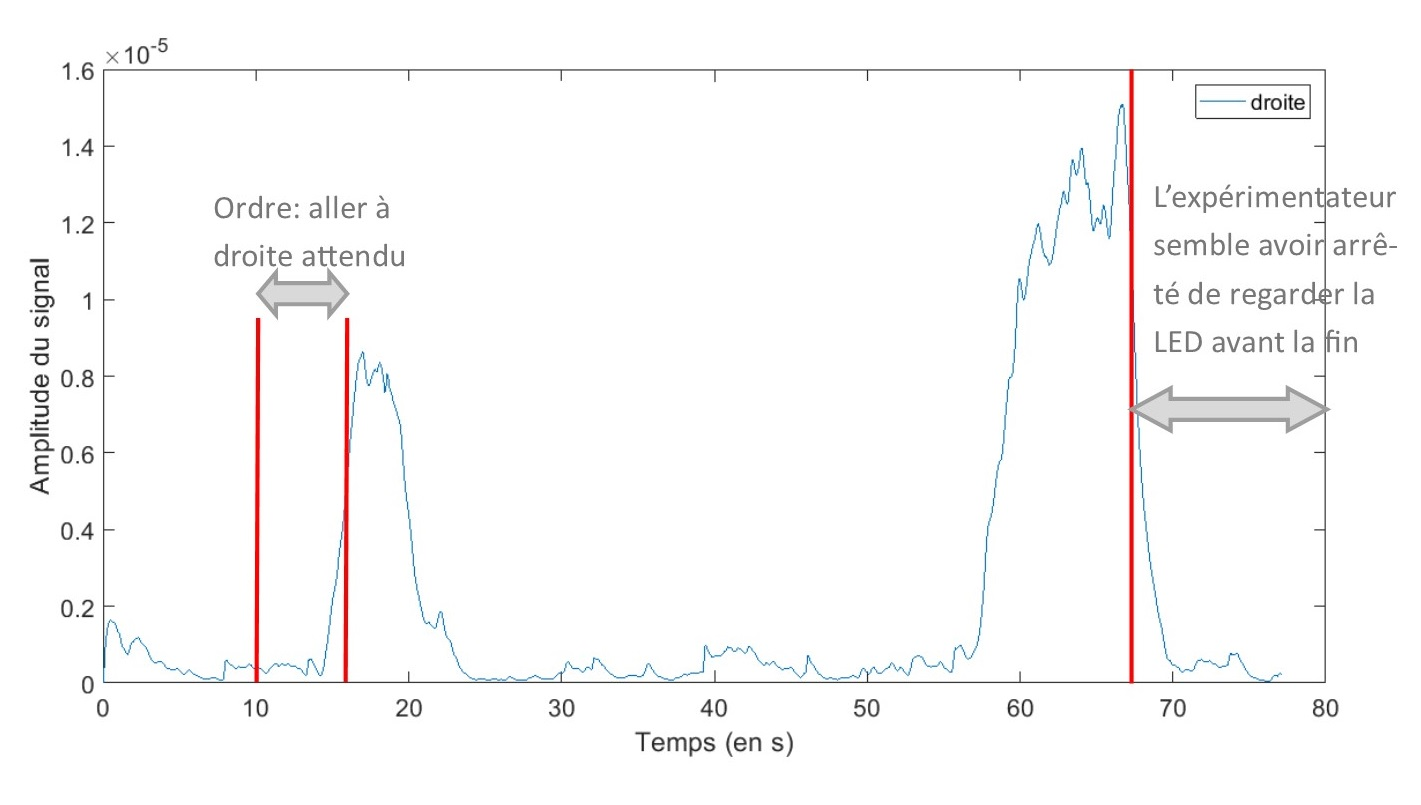
\includegraphics[scale=0.75]{images/herve001corect.jpg}
	\caption{Explications quant aux mauvaises performances du premier enregistrement}
	\label{fig:duck}
\end{figure}

L'image ci-dessous résume les deux explications à ce mauvais résultat. La première explication est que le signal mesuré semble décalé d'environ 4 secondes par rapport à ce qui est attendu. La figure illustre cela uniquement avec la commande "tourner à droite", mais le même constat peut être fait sur les autres commandes. La seconde explication est qu'à la toute fin de l'enregistrements, nous attendons la commande "tourner à droite", or l'expérimentateur semble avoir arrêté de regarder la LED clignotante pendant les quinze dernières secondes avant de terminer l'enregistrement. \\


Ce que nous avons donc fait, c'est que nous avons décalé les labels de 4s et tronqué les 15 dernières secondes du signal. Nous avons ensuite recalculé l'erreur pour ce nouveau signal et le résultat est bien meilleur. En effet, nous avions une erreur auparavant d'environ 55\% et avec le signal modifié, nous avons diminué l'erreur de 28\% pour atteindre les 27\% d'erreur.


\import{/}{signauxopt}

\cleardoublepage

%%%Commande du robot%%%

\import{/}{ROS}
\cleardoublepage
\section{Conclusion}
\cleardoublepage


\end{document}
